\documentclass[11pt]{article}
\usepackage{geometry}                % See geometry.pdf to learn the layout options. There are lots.
\geometry{a4paper}                   % ... or a4paper or a5paper or ... 
\usepackage{graphicx}
\usepackage{amssymb}
\usepackage{url}
\usepackage{listings}
\usepackage{color}

\renewcommand{\textfraction}{0.15}
\renewcommand{\topfraction}{0.85}
\renewcommand{\bottomfraction}{0.65}
\renewcommand{\floatpagefraction}{0.60}

\usepackage{fontspec,xltxtra,xunicode}
\defaultfontfeatures{Mapping=tex-text}
\setromanfont[Mapping=tex-text]{Georgia}
\setsansfont[Scale=MatchLowercase,Mapping=tex-text]{Tahoma}
\setmonofont[Scale=MatchLowercase]{Courier New}


\title{IEG4180 Project 2\\NetProbe Report}
\author{GUAN Hao\\05569511\\hguan5@ie.cuhk.edu.hk}
\date{\today}
\begin{document}
\maketitle
\section{Experiment and Result}
\subsection{Using Blocking I/O}
According to the project specification, I did the experiment by using my own program. The experiment results is shown below.

\begin{figure}
\centering
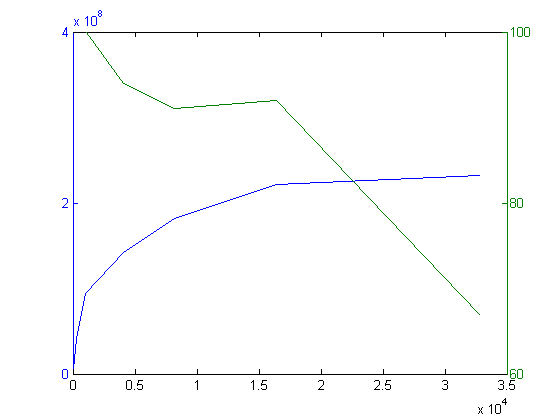
\includegraphics[width=3in]{tcp-blocking.png}
\caption{TCP with blocking I/O.}
\label{fig:TCP}
\end{figure}

\begin{figure}
\begin{minipage}[c]{0.5\textwidth} 
\centering 
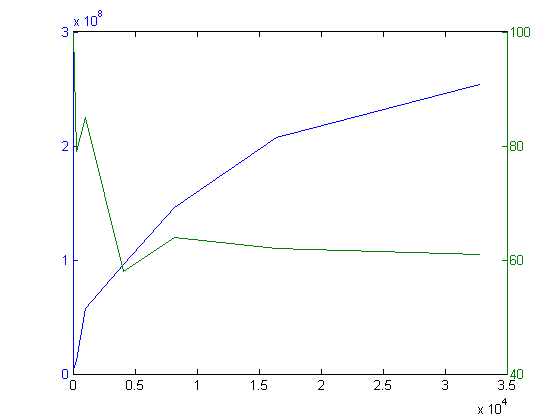
\includegraphics[width=3in]{udp-blocking.png} 
\end{minipage}% 
\begin{minipage}[c]{0.5\textwidth} 
\centering 
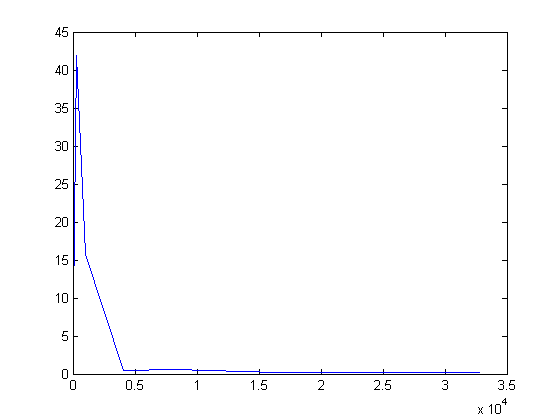
\includegraphics[width=3in]{udp-blocking-lost.png}
\end{minipage}% 
\caption{UDP with blocking I/O.}
\label{fig:TCP}
\end{figure}

\subsection{Using Message-Driven I/O}
\begin{figure}
\centering
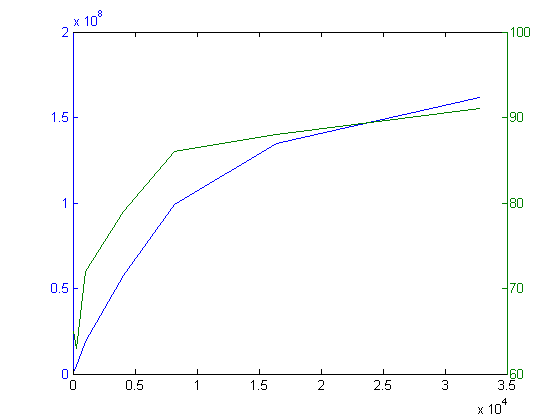
\includegraphics[width=3in]{tcp-msg.png}
\caption{TCP with Message-Driven I/O.}
\label{fig:TCP}
\end{figure}

\begin{figure}
\begin{minipage}[c]{0.5\textwidth} 
\centering 
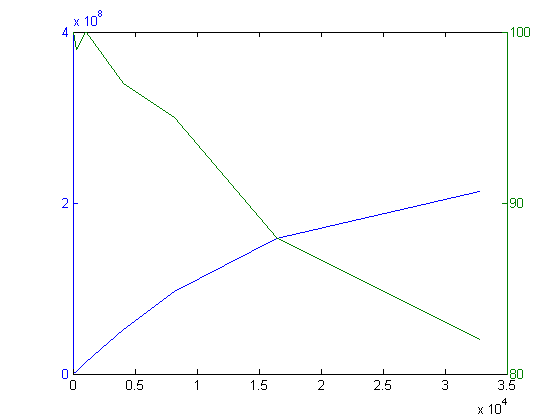
\includegraphics[width=3in]{udp-msg.png} 
\end{minipage}% 
\begin{minipage}[c]{0.5\textwidth} 
\centering 
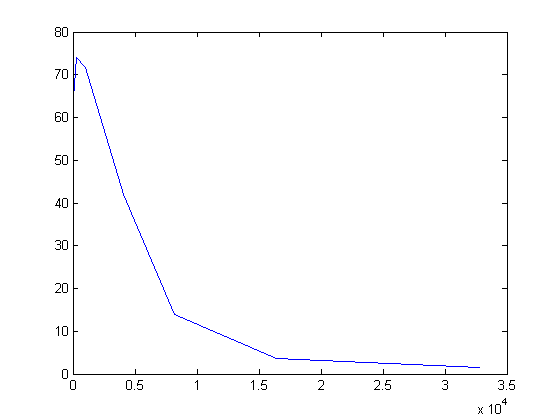
\includegraphics[width=3in]{udp-msg-lost.png}
\end{minipage}% 
\caption{UDP with Message-Driven I/O.}
\label{fig:TCP}
\end{figure}

\section{Experiments on different number of client sessions}
%\begin{table}
\subsection{TCP with blocking I/O}
\begin{center}
\begin{tabular}{cc}
Number of Clients & Max Transmission Rate(Bps) \\ [0.5ex]
\hline\hline
1 & 94345473 \\
2 & 40075632 \\
3 & 21690753 \\
\hline
\end{tabular}
\end{center}

\subsection{TCP with Message-Driven I/O}
\begin{center}
\begin{tabular}{cc}
Number of Clients & Max Transmission Rate(Bps) \\ [0.5ex]
\hline\hline
1 & 18607328 \\
2 & 9535787 \\
3 & 687234\\
\hline
\end{tabular}
\end{center}

\subsection{UPD with blocking I/O}
\begin{center}
\begin{tabular}{cc}
Number of Clients & Max Transmission Rate(Bps) \\ [0.5ex]
\hline\hline
1 & 57321586 \\
2 & 30532488 \\
3 & 6534853 \\
\hline
\end{tabular}
\end{center}

\subsection{UDP with Message-Driven I/O}
\begin{center}
\begin{tabular}{cc}
Number of Clients & Max Transmission Rate(Bps) \\ [0.5ex]
\hline\hline
1 & 11654321 \\
2 & 5314887 \\
3 & 3245783 \\
\hline
\end{tabular}
\end{center}
\section{Declaration}
I declare that the assignment here submitted is original except for source material explicitly acknowledged, and that the same or related material has not been previously submitted for another course. I also acknowledge that I am aware of University policy and regulations on honesty in academic work, and of the disciplinary guidelines and procedures applicable to breaches of such policy and regulations, as contained in the website \url{http://www.cuhk.edu.hk/policy/academichonesty/}
\end{document}
